\begin{frame}{Les termes}
  \begin{columns}
    \begin{column}{0.65\textwidth}
      \begin{block}{}
        \begin{itemize}[<+->]
        \item Des symboles d'arité fixe : $f^{\backslash 2}$
        \item Un alphabet : $\{ a^{\backslash 0}, b^{\backslash 0}, s^{\backslash 1}, h^{\backslash 1}, f^{\backslash 2}\}$
        \item Un terme : $f(f(s(a), a),s(f(b,b)))$
        \end{itemize}
      \end{block}
    \end{column}
    \begin{column}{0.35\textwidth}
      \onslide<4>
      \begin{center}
        \begin{tikz}
          \node {$f$}
          child { node {$f$}
            child { node {$s$}
              child { node {$a$} } }
            child { node {$a$} } }
          child { node {$s$}
            child {node {$f$}
              child { node {$b$} }
              child { node {$b$} } } };
        \end{tikz}
      \end{center}
    \end{column}
  \end{columns}
\end{frame}

\begin{frame}{Langages formels}
  Un ensemble de termes
  \begin{block}{}
    \begin{itemize}[<+->]
    \item Langages réguliers : $\{f(s^*(a),s^*(a))\}$
    \item Langages synchronisés : $\{f(s^n(a),s^n(a)) \mid n \geq 0\}$
    \item Langages algébriques : $\{s^n(h^n(a)) \mid n \geq 0\}$
    \item Langages synchronisés algébriques : $\{f(s^n(h^n(a)),s^n(h^n(b))) \mid n \geq 0\}$
    \end{itemize}
  \end{block}
  \vspace{\baselineskip}
  \begin{overprint}
    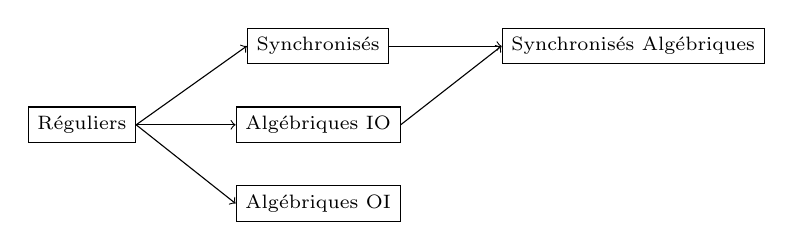
\begin{tikzpicture}

      \tikzstyle{language} = [shape=rectangle, draw];
      
      \onslide<1->{
        \node[language] (reg) at (0,0) {\scriptsize{Réguliers}};
      }

      \onslide<2->{
        \node[language] (synch) at (3,1) {\scriptsize{Synchronisés}};
        \draw[->] (reg.east) -- (synch.west);
      }

      \onslide<3->{
        \node[language] (algeio) at (3,0) {\scriptsize{Algébriques IO}};
        \node[language] (algeoi) at (3,-1) {\scriptsize{Algébriques OI}};
        \draw[->] (reg.east) -- (algeio.west);
        \draw[->] (reg.east) -- (algeoi.west);
      }

      \onslide<4->{
        \node[language] (synchalge) at (7,1) {\scriptsize{Synchronisés Algébriques}};
        \draw[->] (synch.east) -- (synchalge.west);
        \draw[->] (algeio.east) -- (synchalge.west);
      }
    \end{tikzpicture}
  \end{overprint}
\end{frame}

\begin{frame}{Variables}
  \begin{columns}
    \begin{column}{0.6\textwidth}
      \begin{block}{}
        \begin{itemize}
        \item<1-> Ensemble de variables : $\mathcal X = \{x, y\}$
        \item<2-> La substitution : \color<2-3>{focusColor}{$\sigma = (x / s(b))$}
        \item<4-> Le filtrage : \color<5>{focusColor}{$\sigma(t) = t'$}
        \item<6-> L'unification : \color<7>{focusColor}{$\alpha(t) = \alpha(t')$}
        \end{itemize}
      \end{block}
    \end{column}
    \begin{column}{0.4\textwidth}
      \begin{overprint}
        \onslide<2>
        \begin{center}
          \begin{tikzpicture}

            \tikzstyle{focusedNode} = [focusColor];
            
            \node (f) at (0,0) {$f$};
            \node[focusedNode] (x) at (-1,-1) {$x$};
            \node (s) at (1,-1) {$s$};
            \node (a) at (1,-2) {$a$};

            \draw[thick] (f) -- (x);
            \draw[thick] (f) -- (s);
            \draw[thick] (s) -- (a);
          \end{tikzpicture}
        \end{center}
        \onslide<3>
        \begin{center}
          \begin{tikzpicture}

            \tikzstyle{focusedNode} = [focusColor];
            \tikzstyle{focusedEdge} = [focusColor,thick];
            
            \node (f) at (0,0) {$f$};
            \node (s) at (1,-1) {$s$};
            \node (a) at (1,-2) {$a$};
            \node[focusedNode] (sbis) at (-1,-1) {$s$};
            \node[focusedNode] (b) at (-1,-2) {$b$};
            

            \draw[thick] (f) -- (x);
            \draw[thick] (f) -- (s);
            \draw[thick] (s) -- (a);
            \draw[thick] (f) -- (sbis);
            \draw[focusedEdge] (sbis) -- (b);
          \end{tikzpicture}
        \end{center}
        \onslide<4>
        \begin{center}
          \begin{tikzpicture}

            \tikzstyle{focusedNode} = [focusColor];
            
            \node (f) at (0,0) {$f$};
            \node (x) at (-1,-1) {$x$};
            \node (s) at (1,-1) {$s$};
            \node (a) at (1,-2) {$a$};

            \draw[thick] (f) -- (x);
            \draw[thick] (f) -- (s);
            \draw[thick] (s) -- (a);
          \end{tikzpicture}
          \begin{tikzpicture}

            \tikzstyle{focusedNode} = [focusColor];
            \tikzstyle{focusedEdge} = [focusColor,thick];
            
            \node (f) at (0,0) {$f$};
            \node (s) at (1,-1) {$s$};
            \node (a) at (1,-2) {$a$};
            \node (sbis) at (-1,-1) {$s$};
            \node (b) at (-1,-2) {$b$};
            

            \draw[thick] (f) -- (x);
            \draw[thick] (f) -- (s);
            \draw[thick] (s) -- (a);
            \draw[thick] (f) -- (sbis);
            \draw[thick] (sbis) -- (b);
          \end{tikzpicture}
        \end{center}
        \onslide<5>
        \begin{center}
          \begin{tikzpicture}

            \tikzstyle{focusedNode} = [focusColor];
            
            \node (f) at (0,0) {$f$};
            \node[focusedNode] (x) at (-1,-1) {$x$};
            \node (s) at (1,-1) {$s$};
            \node (a) at (1,-2) {$a$};

            \draw[thick] (f) -- (x);
            \draw[thick] (f) -- (s);
            \draw[thick] (s) -- (a);
          \end{tikzpicture}
          \begin{tikzpicture}

            \tikzstyle{focusedNode} = [focusColor];
            \tikzstyle{focusedEdge} = [focusColor,thick];
            
            \node (f) at (0,0) {$f$};
            \node (s) at (1,-1) {$s$};
            \node (a) at (1,-2) {$a$};
            \node[focusedNode] (sbis) at (-1,-1) {$s$};
            \node[focusedNode] (b) at (-1,-2) {$b$};
            

            \draw[thick] (f) -- (x);
            \draw[thick] (f) -- (s);
            \draw[thick] (s) -- (a);
            \draw[thick] (f) -- (sbis);
            \draw[focusedEdge] (sbis) -- (b);
          \end{tikzpicture}
        \end{center}
        \onslide<6>
        \begin{center}
          \begin{tikzpicture}

            \tikzstyle{focusedNode} = [focusColor];
            
            \node (f) at (0,0) {$f$};
            \node[focusedNode] (x) at (-1,-1) {$x$};
            \node (s) at (1,-1) {$s$};
            \node (a) at (1,-2) {$a$};

            \draw[thick] (f) -- (x);
            \draw[thick] (f) -- (s);
            \draw[thick] (s) -- (a);
          \end{tikzpicture}
          \begin{tikzpicture}

            \tikzstyle{focusedNode} = [focusColor];
            \tikzstyle{focusedNode2} = [focusColorBis];
            
            \node (f) at (0,0) {$f$};
            \node (s) at (-1,-1) {$s$};
            \node (b) at (-1,-2) {$b$};
            \node[focusedNode2] (y) at (1,-1) {$y$};

            \draw[thick] (f) -- (y);
            \draw[thick] (f) -- (s);
            \draw[thick] (s) -- (b);
          \end{tikzpicture}
        \end{center}
        \onslide<7>
        \begin{center}
          \begin{tikzpicture}

            \tikzstyle{focusedNode} = [focusColor];
            
            \node (f) at (0,0) {$f$};
            \node[focusedNode] (x) at (-1,-1) {$x$};
            \node (s) at (1,-1) {$s$};
            \node (a) at (1,-2) {$a$};

            \draw[thick] (f) -- (x);
            \draw[thick] (f) -- (s);
            \draw[thick] (s) -- (a);
          \end{tikzpicture}
          \begin{tikzpicture}

            \tikzstyle{focusedNode} = [focusColor];
            \tikzstyle{focusedNode2} = [focusColorBis];
            
            \node (f) at (0,0) {$f$};
            \node (s) at (-1,-1) {$s$};
            \node (b) at (-1,-2) {$b$};
            \node[focusedNode2] (y) at (1,-1) {$y$};

            \draw[thick] (f) -- (y);
            \draw[thick] (f) -- (s);
            \draw[thick] (s) -- (b);
          \end{tikzpicture}
          $\alpha = (\color{focusColor}{x/s(b)}, \color{focusColorBis}{y/s(a)})$\\
          \begin{tikzpicture}

            \tikzstyle{focusedNode} = [focusColor];
            \tikzstyle{focusedEdge} = [focusColor,thick];
            \tikzstyle{focusedNode2} = [focusColorBis];
            \tikzstyle{focusedEdge2} = [focusColorBis,thick];
            
            \node (f) at (0,0) {$f$};
            \node[focusedNode2] (s) at (1,-1) {$s$};
            \node[focusedNode2] (a) at (1,-2) {$a$};
            \node[focusedNode] (sbis) at (-1,-1) {$s$};
            \node[focusedNode] (b) at (-1,-2) {$b$};
            

            \draw[thick] (f) -- (x);
            \draw[thick] (f) -- (s);
            \draw[focusedEdge2][thick] (s) -- (a);
            \draw[thick] (f) -- (sbis);
            \draw[focusedEdge] (sbis) -- (b);
          \end{tikzpicture}
        \end{center}
      \end{overprint}
    \end{column}
  \end{columns}
\end{frame}

\begin{frame}{Systèmes de réécriture}
  \begin{block}{Règle de réécriture}
    \begin{itemize}[<+->]
    \item $l$ et $r$ des termes
    \item $r$ n'est pas une variable
    \item $Var(r) \subseteq Var(l)$
    \item $l \rightarrow r$ est une règle de réécriture
    \end{itemize}
  \end{block}
  \begin{center}
    \onslide<5->
    $\color<7>{focusColorBis}{s(x)}$ $\rightarrow$ $\color<8>{focusColorBis}{s(s(x))}$\\
    \onslide<7->
    $\color<9>{focusColor}{\sigma = (x / a)}$\\
    \onslide<5->
    \begin{overprint}
      \onslide<6>
      \begin{center}
        \begin{tikzpicture}

          \tikzstyle{focusedNode} = [focusColor];
          
          \node (f) at (0,0) {$f$};
          \node (b) at (-1,-1) {$b$};
          \node (s) at (1,-1) {$s$};
          \node (a) at (1,-2) {$a$};

          \draw[thick] (f) -- (b);
          \draw[thick] (f) -- (s);
          \draw[thick] (s) -- (a);
        \end{tikzpicture}
      \end{center}
      \onslide<7>
      \begin{center}
        \begin{tikzpicture}

          \tikzstyle{focusedNode} = [focusColor];
          \tikzstyle{focusedEdge} = [focusColor,thick];
          \tikzstyle{focusedNode2} = [focusColorBis];
          \tikzstyle{focusedEdge2} = [focusColorBis,thick];
          
          \node (f) at (0,0) {$f$};
          \node (b) at (-1,-1) {$b$};
          \node[focusedNode] (s) at (1,-1) {$s$};
          \node[focusedNode] (a) at (1,-2) {$a$};
          \node[focusedNode2] (rws) at (1.5,-1) {$s$};
          \node[focusedNode2] (rwx) at (1.5,-2) {$x$};

          \draw[thick] (f) -- (b);
          \draw[thick] (f) -- (s);
          \draw[focusedEdge] (s) -- (a);
          \draw[focusedEdge2] (rws) -- (rwx);
        \end{tikzpicture}
      \end{center}
      \onslide<8>
      \begin{center}
        \begin{tikzpicture}

          \tikzstyle{focusedNode} = [focusColor];
          \tikzstyle{focusedEdge} = [focusColor,thick];
          \tikzstyle{focusedNode2} = [focusColorBis];
          \tikzstyle{focusedEdge2} = [focusColorBis,thick];
          
          \node (f) at (0,0) {$f$};
          \node (b) at (-1,-1) {$b$};
          \node[focusedNode2] (rws) at (1,-1) {$s$};
          \node[focusedNode2] (rwss) at (1,-2) {$s$};
          \node[focusedNode2] (rwx) at (1,-3) {$x$};

          \draw[thick] (f) -- (b);
          \draw[thick] (f) -- (rws);
          \draw[focusedEdge2] (rws) -- (rwss);
          \draw[focusedEdge2] (rwss) -- (rwx);
        \end{tikzpicture}
      \end{center}
      \onslide<9>
      \begin{center}
        \begin{tikzpicture}

          \tikzstyle{focusedNode} = [focusColor];
          \tikzstyle{focusedEdge} = [focusColor,thick];
          \tikzstyle{focusedNode2} = [focusColorBis];
          \tikzstyle{focusedEdge2} = [focusColorBis,thick];
          
          \node (f) at (0,0) {$f$};
          \node (b) at (-1,-1) {$b$};
          \node (rws) at (1,-1) {$s$};
          \node (rwss) at (1,-2) {$s$};
          \node[focusedNode] (rwa) at (1,-3) {$a$};

          \draw[thick] (f) -- (b);
          \draw[thick] (f) -- (rws);
          \draw[thick] (rws) -- (rwss);
          \draw[thick] (rwss) -- (rwa);
        \end{tikzpicture}
      \end{center}
    \end{overprint}
  \end{center}
\end{frame}
